\mbox{}\\
\vspace{8cm}


This chapter is a reproduction of the following manuscript to be submitted for publication in eLife:

C. I. Mendes, E. Griffiths, A. Manuele, D. Fornika, S. Tausch, T. Le-Viet, J. Phelan, C. Meehan, A. Raphenya, B. Alcock, E. Culp, A. McArthur, M. Feldgarden, G. Tyson, M. Galas, J. Campos, A. Witney, D. Aanensen, A. Black, L. Katz, P. Oluniyi, I. Olawoye, R. Timme, A. T. Vasconcelos, A. Page, D. MacCannell, F. Maguire. 
hAMRonization: Enhancing antimicrobial resistance prediction using PHA4GE standards and specification. 

As discussed in Chapters \ref{ch:introduction} \ref{ch:paper1} and \ref{ch:paper2}, \ac{SMg} can offer relatively unbiased pathogen detection and characterisation, potentially able to provide antimicrobial resistance and virulence profiling in a single methodological step. The rise of \ac{AMR} poses a major threat to human health worldwide.

Despite the relative standardisation of the process to acquire genomic data, either through \ac{WGS} or \ac{SMg}, there's a myriad of different tools available to perform \textit{in silico} \ac{AMR} detection, with some using their own reference database and each one generating a unique, non-standardised report of the genes or variants that can possibly confer resistance in a given sample. This is a huge barrier to the comparison
of results and the modularity of tools within bioinformatic workflows.

In this chapter, we present a standardised output specification for the reporting of genes or variants potentially conferring \ac{AMR}. This specification aims to standardise the reporting of these results, regardless of the tool and/or database used. To ease its utilisation, we've packaged this specification into hAMRonization, a command-line utility that is able to aggregate results from a wide variety of \ac{AMR} detection tools, both species-agnostic and species-specific, providing a unified report tabular form, JSON or through an interactive HTML file that can be opened within the browser for navigable data exploration. 

We aim that with hAMRonization, stakeholders, such as clinical practitioners, will be more efficiently informed of potential \ac{AMR} genes of variants in a given dataset containing genomic information. Ultimately, the possibility of using multiple \ac{AMR} detection tools, with multiple \ac{AMR} databases, increases evidence, which increases confidence in the results obtained. Likewise, differences in databases can be evidenced for better interpretability. 

My contribution to this publication included the development of the antimicrobial detection contextual data specification package, including its conversion and availability in a machine-applicable JSON format. It also includes the design and implementation of the hAMRonization package, results analysis, manuscript production and editing. 

\cleardoublepage 

\begin{center}
\large
\textbf{hAMRonization: Enhancing antimicrobial resistance  prediction using PHA4GE standards and specification}
\end{center}

Catarina I. Mendes$^{1,*}$, 
Emma J. Griffiths$^{2,*}$, 
Alex Manuele$^3$, 
Dan Fornika$^4$, 
Simon H. Tausch$^5$, 
Thanh Le-Viet $^6$, 
Amogelang R. Raphenya$^7$, 
Brian Alcock$^7$, 
Elizabeth Culp$^7$, 
Andrew G. McArthur$^7$, 
Michael Feldgarden$^8$, 
Gregory H. Tyson$^9$, 
Marcelo Galas$^{10}$, 
Josefina Campos$^{11}$, 
Adam A. Witney$^{12}$, 
David M. Aanensen$^{13,14}$, 
Allison Black$^{15}$, 
Emma Hodcroft$^{16,17}$, 
Lee S. Katz$^{18,19}$, 
Paul E. Oluniyi$^{20,21}$, 
Idowu B. Olawoye$^{20,21}$, 
Ruth E. Timme$^{22}$, 
Ana Tereza R. Vasconcelos$^{23}$, 
Andrew J. Page$^6$, 
Duncan R. MacCannell$^{19}$, 
Finlay Maguire$^3$
on behalf of the Public Health Alliance for Genomic Epidemiology (PHA4GE) consortium Data Structures Working Group

$^1$Instituto de Microbiologia, Instituto de Medicina Molecular, Faculdade de Medicina, Universidade de Lisboa, Lisboa, Portugal 

$^2$  Faculty of Health Sciences, Simon Fraser University, Burnaby, BC, Canada

$^3$ Faculty of Computer Science, Dalhousie University, NS, Canada

$^4$ British Columbia Centre for Disease Control, Vancouver, BC, Canada

$^5$ Department of Biological Safety, German Federal Institute for Risk Assessment, 10589 Berlin, Germany

$^6$ Quadram Institute, Norwich, UK

$^7$ Department of Biochemistry and Biomedical Sciences and the Michael G. DeGroote Institute for Infectious Disease Research, McMaster University; Hamilton; Ontario; Canada

$^8$ National Center for Biotechnology Information, National Library of Medicine, National Institutes of Health; Bethesda; Maryland; USA

$^9$ Center for Veterinary Medicine, U.S. Food and Drug Administration; Laurel; Maryland; USA

$^{10}$ Communicable Diseases and Environmental Determinants of Health, Pan American Health Organization; Washington DC; USA

$^{11}$ INEI-ANLIS "Dr Carlos G. Malbrán"; Buenos Aires;  Argentina

$^{12}$ Institute for Infection and Immunity, St George’s, University of London; London; UK

$^{13}$ Centre for Genomic Pathogen Surveillance, Wellcome Genome Campus; Cambridge; UK; 

$^{14}$ The Big Data Institute, Li Ka Shing Centre for Health Information and Discovery, Nuffield Department of Medicine, University of Oxford; Oxford; UK

$^{15}$ Department of Epidemiology, University of Washington; Washington; USA.

$^{16}$ Biozentrum, University of Basel, Basel, Switzerland

$^{17}$ Swiss Institute of Bioinformatics; Lausanne; Switzerland

$^{18}$ Center for Food Safety, University of Georgia; Georgia; USA; 

$^{19}$ National Center for Emerging and Zoonotic Infectious Diseases, Centers for Disease Control and Prevention; Georgia; USA

$^{20}$ African Center of Excellence for Genomics of Infectious Diseases (ACEGID), Redeemer's University, Ede; Osun State; Nigeria; 

$^{21}$ Department of Biological Sciences, College of Natural Sciences, Redeemer's University; Ede; Osun State; Nigeria

$^{22}$ Center for Food Safety and Applied Nutrition, U.S. Food and Drug Administration; College Park; MD; USA

$^{23}$ Bioinformatics Laboratory National Laboratory of Scientific Computation LNCC/MCTI; Rio de Janeiro; Brazil

$^*$ Contributed equally 

\section{Abstract}

The detection of antimicrobial resistance (AMR) directly from genomic or metagenomic data has become a standard procedure in public health, with a large number of different bioinformatic tools currently available to perform this task. These tools, although implementing similar principles, differ in supported inputs, search algorithms, parameterisation, and underlying reference databases. Each of these tools generates a report of detected AMR genes or variants in a distinct, non-standard, format. This is a huge barrier to the comparison of results and the modularity of tools within bioinformatic workflows. 

The Public Health Alliance for Genomic Epidemiology (PHA4GE) (\url{https://pha4ge.org}) has developed a standardized output specification for the bioinformatic detection of AMR from genomes. hAMRonization, a python package and command-line utility, implements PHA4GE’s AMR specification to combine the outputs of disparate antimicrobial resistance gene detection tools into a single unified format.  hAMRonization can be easily extended, currently supporting 18 different tools, both species-agnostic and species-specific, for the detection of genes and/or variants conferring AMR. The harmonized reports are available in tabular form, JSON or through an interactive HTML file that can be opened within the browser for navigable data exploration. The hAMRonization and underlying specification are open-source and freely available through PyPI, conda and GitHub (\url{https://github.com/pha4ge/hAMRonization}).

\subsubsection{Keywords}

interoperability; antimicrobial resistance; public health; workflows

\section{Introduction}

Antimicrobial resistance (AMR) represents a present and growing public health crisis with a global impact. Multidrug resistance is increasing in a broad range of pathogens \cite{aslam_antibiotic_2018}; combined with low rates of antimicrobial drug discovery \cite{brown_antibacterial_2016} this represents a threat to human and animal health \cite{who_who_2015}. National and international action plans e.g., \cite{jim_oneill_antimicrobial_2014, jim_oneill_tackling_2016,public_health_agency_of_canada_antimicrobial_2014,who_who_2015}, have identified several strategies to mitigate the risk of AMR such as rapid diagnosis of the AMR determinants present within a clinical sample, improved surveillance of AMR, and gaining a better understanding of the mechanisms of environmental AMR transmission.

Diagnostic and public health surveillance analyses are increasingly performed using genomic and metagenomic data \cite{mcarthur_antimicrobial_2017}. Therefore, accurate identification of genes or variants from genomic data which are predicted to confer resistance to antimicrobials is critical for monitoring and attempting to mitigate the spread of AMR. This work is being performed all over the world by public health agencies, clinicians, industry, and academic researchers. Given the scale of this problem and the number of stakeholders involved, many bioinformatics tools have been developed that are dedicated to the task of AMR gene and variant detection \cite{boolchandani_sequencing-based_2019,hendriksen_using_2019,mcarthur_antimicrobial_2017}. There are at least 18 active (as of 2022) open-source command-line tools designed to identify the presence of genes and/or variants associated with AMR.  

These tools include several developed to work with a specific primary database, e.g., the Resistance Gene Identifier (RGI) for the Comprehensive Antibiotic Resistance Database (CARD) \cite{alcock_card_2020}, AMRFinderPlus and the National Center for Biotechnology Information (NCBI) Pathogen Detection Reference Gene catalogue \cite{feldgarden_validating_2019}, and ResFinder and KmerResistance \cite{clausen_benchmarking_2016} for the ResFinder database \cite{zankari_identification_2012}.  Other tools exist that use merged forms of existing databases such as ResFams \cite{gibson_improved_2015}, AMRplusplus \cite{doster_megares_2020}, and DeepARG \cite{arango-argoty_deeparg_2018}. Finally, there are AMR gene identification tools that provide a database-agnostic approach using novel algorithms (e.g., GROOT \cite{rowe_indexed_2018}, ARIBA \cite{hunt_ariba_2017}), or a different interface (e.g., ABRicate \cite{torsten_seeman_abricate_2020}, sraX \cite{panunzi_srax_2020}). 

These tools all have different strengths and weaknesses exist attributable to varied underlying databases, search algorithms, and default parameterisations. Based on the specific requirements of a given AMR analysis context one tool may be better suited to the analytical workflow than another.    
Unfortunately, all these tools also generate differently formatted outputs using divergent terminology. This poses a significant challenge to the effective integration, modularity, and comparison of AMR gene detection methods. The consequence of this is that it is difficult for researchers and public health experts to systematically evaluate the suitability of different tools in their workflow. With the limited examples of these comparisons largely reliant on the development of custom ad-hoc tool-specific parsers, e.g., \cite{feldgarden_validating_2019, hunt_ariba_2017}), or has skipped the tools entirely and directly compared the underlying algorithms e.g., \cite{mccall_comparative_2018}. Even in cases where benchmarking has been performed, the disparate output formats mean it requires significant work to modify a workflow to use a different AMR detection tool. This greatly limits modularity and flexibility to integrate new tools into existing analyses or repurpose them to new or changing requirements.  Given the recent calls to mitigate these issues in public health genomic epidemiology \cite{black_ten_2020}, it is critical that data structures and methods are developed which enable tool-agnostic, robust parsing, manipulation, and transformation of AMR gene detection results.

To this end, we compared and consolidated the outputs of existing AMR gene detection tools to develop the hAMRonization specification. This is a standardised set of recommended and mandatory output terms and labels for AMR gene detection tools, such as “Gene Name”, “\% Coverage (breadth)”, and “Drug Class”.  The outputs for all currently maintained, general purpose, AMR gene detection tools can be directly converted to this unified specification.  Furthermore, this conversion to a common AMR gene detection output specification can be performed automatically using a companion library of  biopython-compatible parsers.

\section{Results}

\subsection{The PHA4GE hAMRonization Detection Specification}

The PHA4GE hAMRonization Detection specification was designed to harmonize information prioritised by public health practitioners for genomic surveillance, outbreak investigations and research with direct public health impacts. Fields from various widely used AMR detection tools were compared, and a set of 36 fields were selected to capture information regarding the software and database provenance, information about reference genes and genomes, as well as mutations and resistance genes detected in sequences of interest. The field labels are standardised using terms sourced or contributed to open-source ontologies. Ontologies are sets of controlled vocabulary arranged in a hierarchy, in which terms are linked using logical relationships and the meanings of the terms are disambiguated by the assignment of unique and persistent identifiers. The positions of detected mutations with respect to reference genes/genomes/proteins are specified using the machine-readable Human Genome Variation Society (HGVS) notation system, a sequence variant nomenclature that has been used previously for encoding tuberculosis drug resistance mutations (den Dunnen et al., 2016). To translate HGVS notations into clinician-friendly, human-readable language, a simplified interpretation of mutation coordinates is also provided within the specification. A list of the fields in the specification, along with their ontology identifiers, definitions, expected value types, examples of use, and additional guidance for implementation, are presented in Table \ref{tab:ch6_table1}. It should be noted that the guidance is meant to provide recommendations for developers and may contain suggestions that go beyond the immediate aims of the specification.

\begin{table}[]
\centering
\caption{hAMRonization: AMR Gene Detection Output Specification.}
\label{tab:ch6_table1}
Table available for download at \url{https://zenodo.org/record/7286376/files/PHA4GE\%20AMR\%20Gene\%20\%26\%20Variant\%20Specification\%20-\%202022.xlsx}
\end{table}

\subsection{hAMRonization Data Transformation, Parsing Tools, and Harmonized Reports}

To enable automated data transformations from variable tool outputs to the PHA4GE hAMRonization specification, fields from 18 gene and mutation detection tools (i.e. ABRicate, AMRFinderPlus, AMRPlusPlus, ARIBA, C-SSTAR, DeepARG, GROOT, KmerResistance, ResFams, ResFinder (includes PointFinder), SraX, SRST2, and StarAMR) were mapped to the specification. It’s worth noting that not all tools provide values for all specification fields. Also, many tools provide outputs beyond what is captured by the specification. 

Parsers were then constructed to automate the transformation and movement of outputs into the appropriate fields in the hAMRonization reports (Figure \ref{fig:chap6_figure1}). Parser code is open source, and all code and installation instructions are available at \url{https://github.com/pha4ge/hAMRonization}. hAMRonization can be executed from the command-line, and alternatively, can be installed and used in Galaxy via the Galaxy tool shed.
hAMRonization provides both tabular and interactive reporting formats. The interactive report provides the user with an HTML file that can be opened within the browser for navigable data exploration.

\begin{figure*}[]
\centering
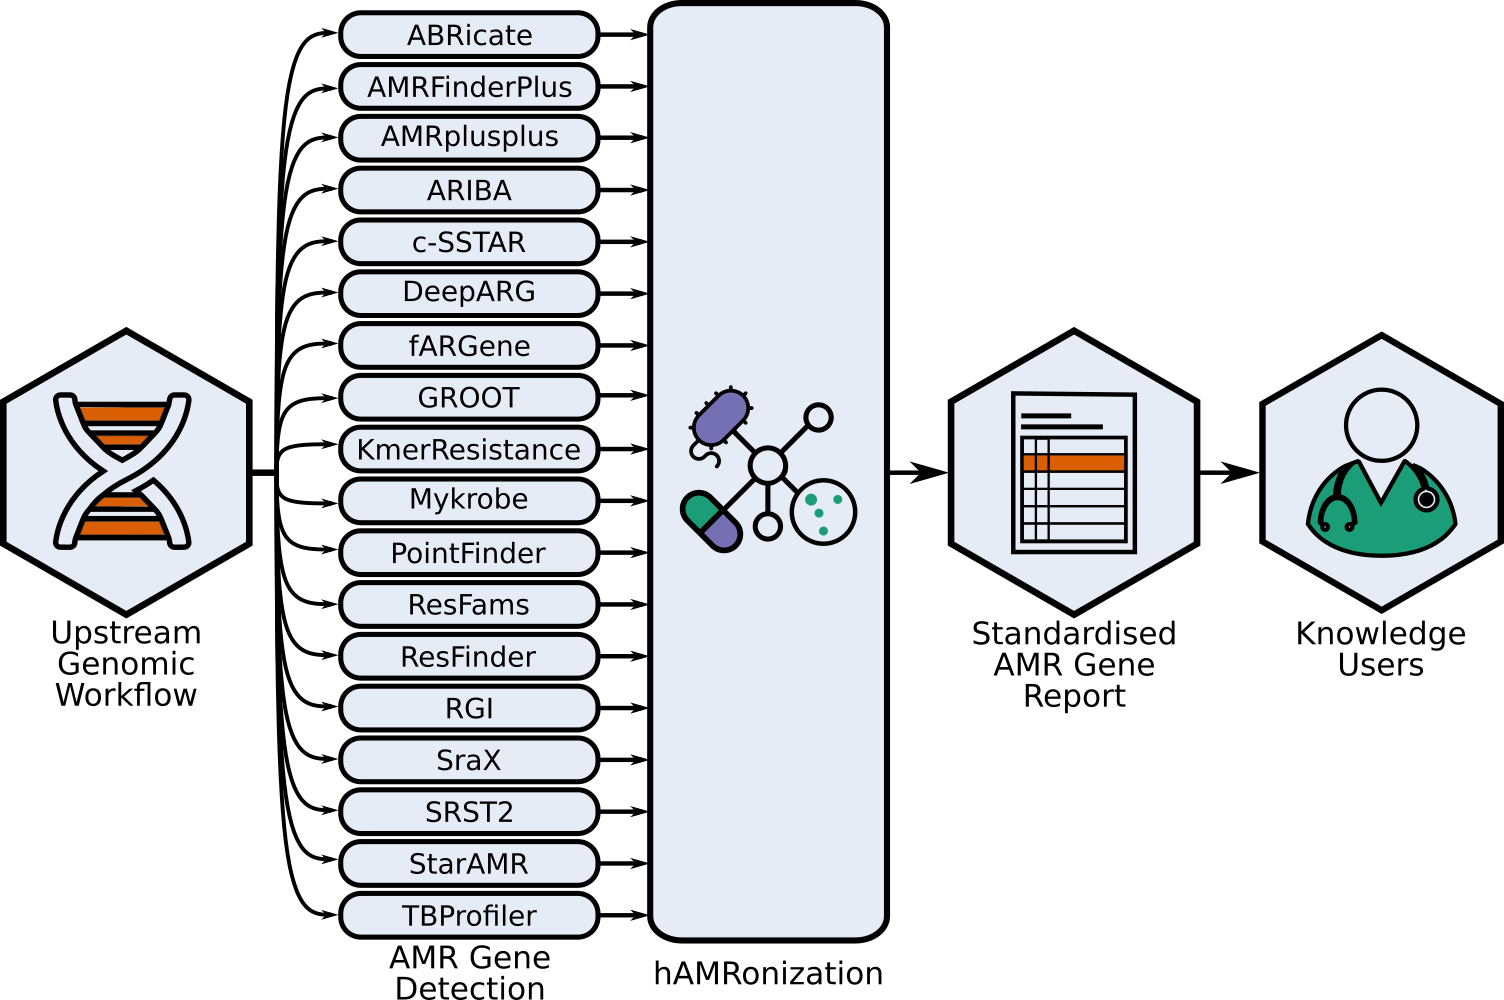
\includegraphics[width=\textwidth]{figures/chapter 6/Fig 1.png}
\caption{ Overview of hAMRonization within standard AMR genomics/metagenomics workflows. The hAMRonization module and command-line utility tools allow the creation of a single unified output report from any of 18 established disparate AMR gene and/or variant prediction tools. This facilitates users such as national public health reference laboratories and academic institutions to compare results across tools and change their workflow to different tools without having to develop custom code.  It also means that the communication of results to downstream knowledge users, such as infection control prevention clinicians, can be done in a consistent standardised manner regardless of which AMR prediction tool was used in the genomic/metagenomic analysis.}
\label{fig:chap6_figure1}
\end{figure*}

\subsection{hAMRonization Snakemake Pipeline}

The developed  hAMRonization snakemake pipeline (see \ref{ch6_materials_workflow}) was used to run two sets of data through a selection of AMR detection tools, using various AMR gene databases. 

\subsection{Piloting hAMRonization in Real-World Public Health Settings}

To test the utility and value of the hAMRonization specification and its associated tools for AMR genomic surveillance and data sharing, pilot projects were launched in laboratories across three partner teams, which included Cambodia/Australia, Nigeria (seven laboratories across the AMR surveillance network), and Malaysia/Argentina via a PHA4GE subgrant competition. PHA4GE also engaged eight labs from seven countries in Latin America via the ReLAVRA AMR surveillance network (a network associated with the Pan American Health Organization (PAHO), a regional office of the World Health Organization). Participants were issued with a short document outlining the purpose of the software, installation instructions and prompting questions for feedback on their experience. Participants were also asked to share harmonized data among their networks where previously sharing was difficult due to the variability of tool outputs. As hAMRonization and its associated materials are written in English, the documentation had to first be translated into Spanish by PAHO prior to distribution in Latin American countries. 

Subgrant participants used hAMRonization to analyse data from hospital settings and/or national surveillance projects involving a variety of organisms e.g. \textit{Salmonella paratyphi}, Methicillin-Resistant \textit{Staphylococcus aureus} (MRSA). Feedback included the need for improved definitions of fields and guidance on required inputs, the need for certain fixes for circumstances causing hAMRonization crashes, and the need for more clinician-friendly installation and execution instructions. Some participants also suggested that the inclusion of sequence contextual data would be helpful for analysis (i.e. hospital name and country of sample collection, ward (medical vs surgical), collection date, specimen type (e.g. blood, urine), latitude/longitude of sample collection). In addition to the testing exercise performed, the Nigeria Team (led by the University of Ibadan) integrated hARMonization into their NextflowTower platform for AMR bioinformatics analysis training workshops. To better enable their clinician colleagues without bioinformatics expertise to use the hAMRonization, the Malaysia/Argentina Team (led by the National University of Malaysia) developed a Google Colaboratory (a Google Notebook that enables code to be executed from a Browser) and has distributed it to their network partners.

The ReLAVRA pilot included National Reference Laboratories from Argentina, Brasil, Chile, Colombia, Costa Rica, México and Paraguay. Laboratories and were provided with a dataset of 20 \textit{Shigella sonnei} genomes from a previous Latin America regional project analysed with 5 different AMR detection tools: ABRIcate, AMRFinderPlus, ARIBA, SRST2, StarAMR. Participants received the outputs of the AMR detection tools together with the instructions for installing and running hAMRonization. When participants completed the exercise, they were asked to complete the structured poll. Twelve responses from the seven participating nations were received, and a summary report was prepared by ReLAVRA and provided to PHA4GE. Most of the participants were bioinformaticians and laboratory technicians. For bioinformaticians, the installation instructions were easy to follow, however, laboratory technicians without a bioinformatics background expressed difficulties largely with the dependencies installation. Participants agreed that all harmonised output fields provided relevant information for AMR detection but the most useful were the fields that cover the AMR gene detected and the confidence of that result. Respondents were concerned about the importance of having knowledge of AMR and genomic data analysis for the correct interpretation of the results, especially with regard to decision-makers in clinical settings. An example related to this concern was that when detecting \textit{blaTEM-1} gene by AMRFinderPlus, the field “antimicrobial agent” indicates "Beta-lactam", but this type of drug includes a wide variety of antibiotics, from amoxicillin to extended-spectrum cephalosporins (ESC) and carbapenems. However, \textit{TEM-1} is an extended-spectrum beta-lactamase that does not confer resistance to ESC or carbapenems. While this concern arises from the output of AMRFinderPlus rather than hAMRonization, this challenge is a barrier to the implementation of genomics for AMR surveillance in clinical settings and should be addressed. PHA4GE is cataloguing such critical challenges and will work with the community to solve them. In terms of output summary format, most of the participants preferred the tabular report, citing that a single file combining all the relevant information was more convenient and amenable to processing with different downstream software. Some participants preferred citing its user-friendly visual interface was helpful for comparing which tools identified the same gene.

While differences in gene nomenclature arise from variability in reference databases, users expressed that harmonization of gene names across different reference databases would be extremely helpful (especially those produced by ARIBA). Fields that require knowledge to interpret should not be included e.g. “antimicrobial agent”. While hAMRonization does not generate the tool-specific error warnings that users sometimes encounter while running the tools, it would be useful to provide explanations of these warnings in the user guide. 

While differences in tool algorithms are outside of the scope of hAMRonization, they result in discrepancies in results which are highlighted by hAMRonization e.g. the absence of a result because the gene was not present in the sequence of interest or due to its absence in the database or due to differences in the search algorithms used by each AMR tool. Users suggested that providing some explanation of the differences in tool algorithms would be helpful for interpretation.

Overall, all users found the tool very useful for doing regional genomic surveillance and sharing results with different laboratories that use different AMR detection tools across networks. Technical issues such as fixes for crashing, improved definitions, and instructions for inputs were addressed. Ways to address bigger picture requests such as the harmonization of gene nomenclature, tool-specific issues, and the inclusion of contextual data (sample metadata as well as epidemiological, clinical and laboratory data) are under discussion by PHA4GE.

\subsection{hAMRonization and Research Analysis and Biological Insights}

To test the utility and value of the hAMRonization specification and its associated tools for biological research, PHA4GE engaged partners from the research community. hAMRonization was used to benchmark tools for the detection of AMR genes in \textit{Klebsiella pneumoniae} by researchers at McMaster University (Hamilton, Canada), and was also used to compare \textit{Pseudomonas aeruginosa} Sequence Types associated with a Metallo-Carbapenemases resistance outbreak in the United Kingdom by researchers at the University of London (London, UK). hAMRonization challenges identified during the pilots were also addressed during an AMR hackathon organised by PHA4GE, CLIMB-Big Data, and the Joint Programming Initiative on Antimicrobial Resistance (JPIAMR).

\subsubsection{\textit{Klebsiella pneumoniae} and tool benchmarking}

A dataset of 89 Klebsiella pneumoniae were analysed using RGI, relying on BLASTp and the CARD database, RGI btw, relying on Bowtie2 and the CARD database, AMRFinderPlus which uses BLASTx and the BARRG database, and ResFinder with BLASTn and the ResFinder database. The aim was to determine the number of unique AMR genes identified, with a large variation having been identified across the four tools (Figure \ref{fig:chap6_figure2}). RGI bwt and RGI identified the highest number of hits (n=223 and n=140 respectively), albeit using different identification methods both use the same database. AMRFinderPlus and Resfinder identified an order of magnitude less AMR genes (n=70 and n=46 respectively), even though both rely on BLAST, as does RGI. This highlights the impact of the database chosen when assessing AMR genes. 

\begin{figure*}[]
\centering
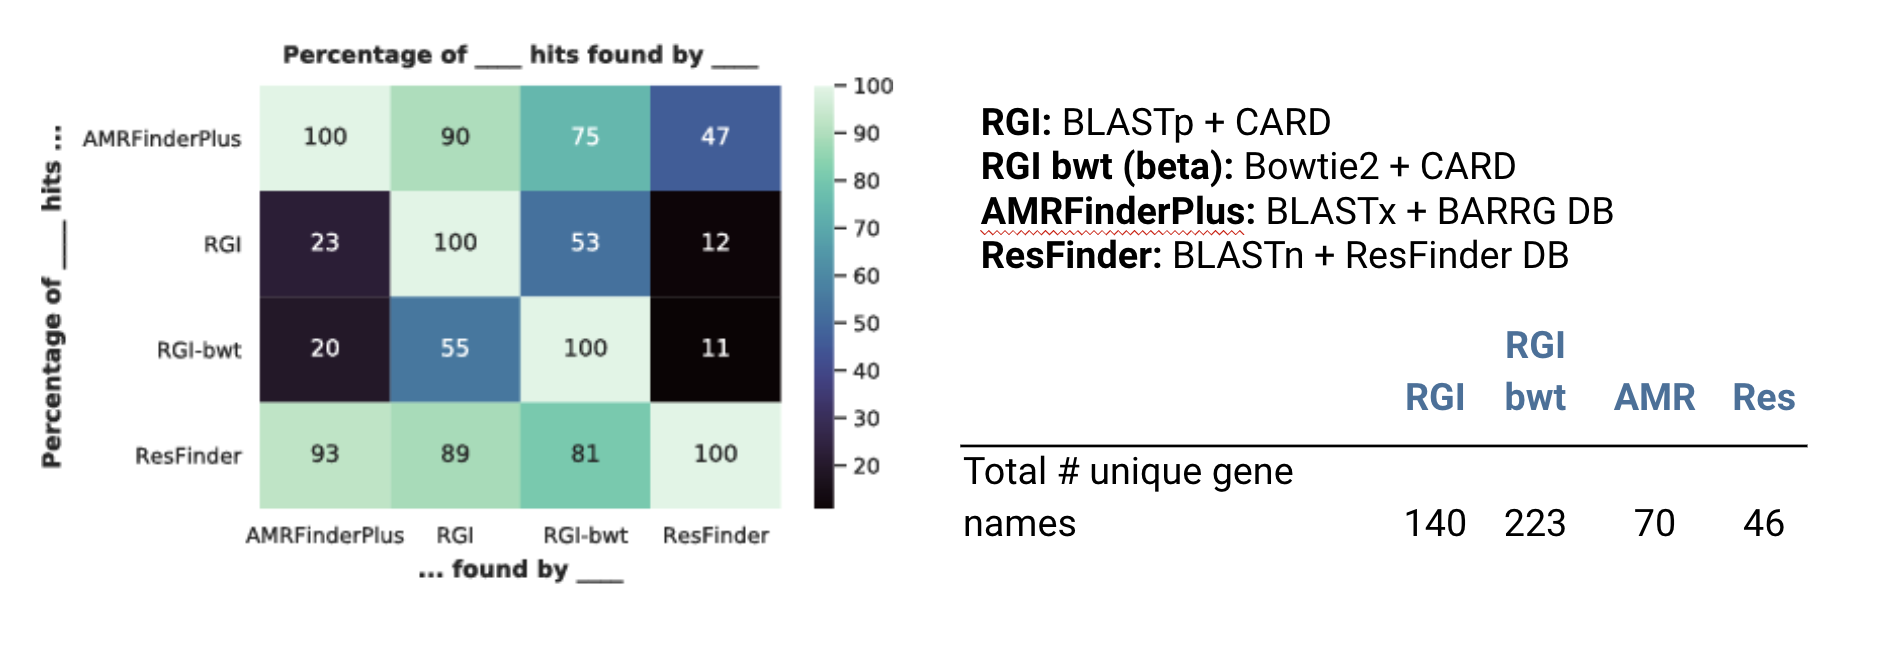
\includegraphics[width=\textwidth]{figures/chapter 6/Fig 2.png}
\caption{Unique AMR genes idenfiied by RGI, RGI bwt, AMRFInderPlus and ResFinder. The heatmap represents the percenetage of AMR genes found by the combination of the four tools. Although a very large percentage of the ResFinder and AMRFinderPlus detected genes are identified by all tools, RGI and in particular RGI bwt identify a very large subset of AMR genes not present in the othe datasets.}
\label{fig:chap6_figure2}
\end{figure*}

\subsubsection{Characterizing \textit{Pseudomonas aeruginosa} Sequence Types associated with Metallo-Carbapenemase resistance in an outbreak}

A set of 87 \textit{Pseudomonas aeruginosa} sequences (ST 111) associated with a Metallo-Carbapenemases resistance outbreak in the United Kingdom \cite{witney_genome_2014}, were analysed using ABRIcate, AMRFinderplus, C-SSTAR, Resfinder, StarAMR with default parameters and databases. The resulting outputs were combined using hAMRonization (Figure \ref{fig:chap6_figure3}). Most isolates (n=73) carried the \textit{VIM-2} gene, conferring the observed resistance phenotype. Some genes, such as \textit{crpP} and \textit{sul1},  are repeatedly identified by most of the tools. Differences in gene nomenclature in different databases complicate comparisons e.g. the same gene was also seen with different spelling, such as \textit{blaVIM-2} being called a \textit{blaVIM}. Nomenclature issues aside, harmonised outputs from different tools served to increase the body of evidence (and confidence in results) indicating the role of different AMR determinants in the outbreak.

\begin{figure*}[]
\centering
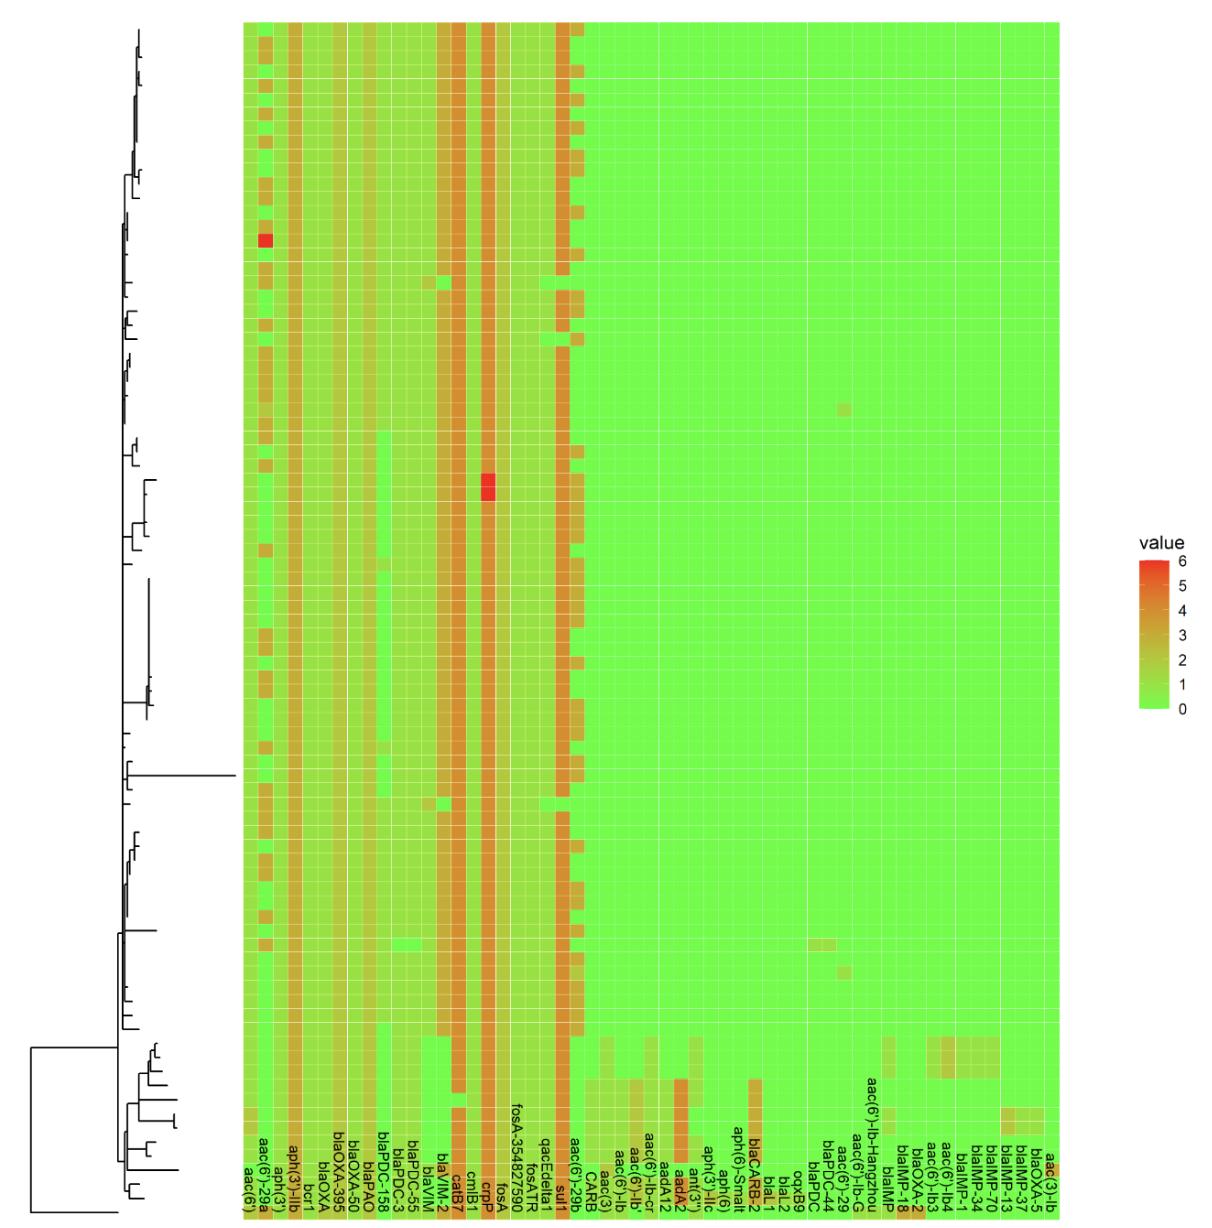
\includegraphics[width=\textwidth]{figures/chapter 6/Fig 3.png}
\caption{Heatmap of the number of predictions made by the AMR gene detection tools (abricate, amrfinderplus, csstar, resfinder, staramr) that find each resistance gene, overlaid on a tree from those isolates.}
\label{fig:chap6_figure3}
\end{figure*}

\subsubsection{hAMRonization and Hackathon-based Community Development}

A hackathon jointly organized by PHA4GE, CLIMB-Big Data, and JPIAMR was held in October 2021 (\url{https://github.com/AMR-Hackathon-2021}). The aim of the hackathon was to improve upon currently available bioinformatics tools and methods for the AMR community, with a special focus on antimicrobial resistance in bacteria. A hackathon is an event in which a large number of people from the community meet to engage in collaborative computer programming. Project ideas are pitched, and participants form working groups based on the projects proposed. PHA4GE representatives pitched challenges identified during the hAMRonization pilot implementations as hackathon projects - such as the need for a clinician-friendly interpretation of HGVS notation and the need for harmonization of gene nomenclature across reference databases. As a result of the collaborative work during the hackathon, the hAMRonization specification was improved by the development of a layman’s translation of HGVS notation specifying the coordinates of mutations identified within genes, proteins and genomic sequences of interest in relation to their position to a reference sequence (led by Dr Connor Mehan, University of Blah). Furthermore, the use of an ontology-based tool for harmonizing gene nomenclature called CHARMdb was explored and tested in hARMonization  (led by Dr Anthony Underwood, previously of Public health England, currently at Broken String Biosciences Ltd). While CHARMdb is not yet fully integrated into hAMRonization, we anticipate its use in future development. These achievements are examples of the important work that can be done when scientists are brought together to use their creativity and expertise to solve problems at community-driven hackathons.

\section{Discussion}

The lack of standardisation in the reporting of AMR gene and mutation detection greatly hinders the comparison of results across the public health sector. The myriad of options available for this purpose highlights a grave interoperability problem. In this work, we have identified and prioritised data elements capturing AMR detection information most pertinent for public health decision-making. We have developed a standardised specification for harmonising variable AMR detection tool outputs, implementing open source, community-based ontologies as well as standardised formats and nomenclatures. We have also operationalised the specification through the development of tools (parsers and workflows) and harmonised reports, available as a package called hAMRonization. We have also tested the hAMRonization in different public health and research settings. The results of this work have shown that hARMonization enables the dissemination of results to stakeholders in a single consistent format, allowing not only the comparison of tools and databases, but the validation of results through multiple detection algorithms. 

The developed standardized data specification and python package and command line utility improve data harmonization and interoperability, allowing the comparison of results not only across multiple AMR detection algorithms but also AMR reference databases. hAMRonization also improves the capture of provenance information, such as the versions of software and databases used in analyses, which can help improve the reproducibility of results. 

It should be noted that while hAMRonization has been applied to AMR detection, many data elements are use case agnostic and so can be repurposed for the detection of genes and mutations associated with other phenotypes such as virulence, pathogenicity, transmissibility, heavy metal resistance, mobility factors etc. Extension of the specification through the adding of other optional higher-order annotation fields such as virulence factor type (“adherence”, “toxin” etc) or metal type, could help to create modularity, different types of detection streams, and feed directly into other downstream analysis. A limitation of hAMRonization currently is that while individual determinants contributing to resistance can be detected however there is no support for highlighting the presence of multi-component resistance mechanisms such as glycopeptide resistance clusters \cite{courvalin_vancomycin_2006} or efflux pumps \cite{okusu_acrab_1996} in this specification.

One of the most substantial challenges with any attempt to improve interoperability by introducing new standards/specifications is their uptake. We have attempted to minimise the barriers to uptake by operationalizing it with a set of automated data transformation tools. For each of the AMR detection tools, a set of  “mappings” or instructions to convert their outputs to the hAMRonization specification has been provided along with parsers to automate this process. Ideally,  developers will adopt this specification and structure their tool’s output accordingly in the future. This would obviate the need for future mappings and parsers. However, even if this does not occur, the nature of the specification means that only minimal effort would be required to convert tabular results from any novel AMR gene detection tool. Another benefit of such a community-based consensus standard for AMR detection is that it provides much-needed standards for industrial partners developing instruments and devices. A challenge within public health laboratories is the lack of interoperability between different phenotype characterization instruments and lab information management systems. Providing community-vetted, standardised specifications for genomics applications enables vendors to develop tools and other resources that are interoperable and add value (for example, an AMR typing platform conforming to the hAMRonization standard could produce results that could more easily plug into a LIMS of other downstream software more seamlessly).

The implementation of hAMRonization in real-world settings has enabled us to more clearly catalogue and articulate public health challenges outside of the scope of the specification and tools, that impact the use of hAMRonization. Lessons learned to include the fact that the harmonization of data for genomic surveillance comes with additional needs outside of standards and technical implementation, including improved support for the interpretation and evaluation of harmonised data. Also, in harmonising the outputs of tools using different computational approaches, the strengths and weaknesses of the tools need to be made more transparent to users as they become removed from working directly with the individual tools themselves. Future work will focus on these areas, as well as better harmonising gene nomenclature across reference databases.

In summary, through the uptake of hAMRonization data standard and associated tools, we aim to improve the comparability of results, and the interoperability of workflows in the public health microbial genomics ecosystem. This will lead to better AMR surveillance, more effective genomic diagnostics, and ultimately improved human and animal health. 

\section{Materials and Methods}

\subsection{PHA4GE hAMRonization Specification}

To compare and unify the broad set of output fields across individual AMR gene detection tools it is necessary to create a common language that can be used to describe them all.  This takes the form of a standardised set of output labels and ontological identifiers (linked to standardised definitions). Individual fields from the output of each tool can then be mapped to a standardised label. For example, the accession of the contig a given AMR gene was detected on is listed as “Contig” in RGI, “contig\_name” in ResFinder, and "contig id" in AMRFinderPlus. Therefore, our specification includes a standardised “Contig ID” field which captures all of these values across tools. 

This common language, or specification, was created through an iterative expert-led process which consisted of curating and comparing output formats from 18 open-source, species-agnostic AMR gene detection tools, with evidence of active use in the literature. This included consultation with an international set of national public health groups, tool developers, and AMR genomics experts through the PHA4GE initiative. In addition to identifying terms compatible with the range of outputs, this work also involved the identification of a core set of essential contextual data for use of AMR  detection in health or research contexts.  This includes items such as the input filename, name and version of the AMR database used, and the name and version of the AMR gene detection tool.  Once the prioritised data elements were selected, definitions and implementation guidance for the standardised fields were developed. Appropriate ontology terms matching the desired data elements were sourced from different OBO Foundry ontologies. Ontologies within the OBO Foundry library are developed using common principles and practices designed to increase interoperability across domains of knowledge. Terms in the draft AMR specification for which ontology concepts already existed were adjusted to align with community standards. Terms which did not already exist were submitted to appropriate source ontologies. Ontologies are meant to represent “universal truth” as much as possible, and not just use case-specific nuances. As such, additional guidance was provided for AMR detection-specific implementation. Fields, definitions, specification-specific guidance, value types, and examples of use can be found in the hAMRonization specification available on GitHub. In total, the specification consists of 36 fields sourced/harmonised with the Ontology for Biological Investigations (OBI), the Antimicrobial Resistance Ontology (ARO), the Genomic Epidemiology Ontology (GenEpiO), and the Chemical Entities of Biological Interest Ontology (ChEBI).  
The finalised hAMRonization specification was then encoded in JSON format to enable automated computer validation of hAMRonized output reports and deposited within the hAMRonization git repository.


\subsection{hAMRonization Package}

Mappings from the output fields in each of the 18 tools to the hAMRonization specification were then encoded in a python package (github.com/pha4ge/hAMRonization). This package was developed following the modular approach of biopython \cite{cock_biopython_2009} and provides an easy-to-use command line tool to enable automatic conversion of output files from each of these tools to a standardised report following the hAMRonization specification. Where appropriate and when tools don’t provide the full set of essential core metadata will prompt for this information to ensure high-quality reproducible analyses.  This tool allows the collation of results from multiple tools and samples into a single standardised report to aid comparison and analysis.  These reports can optionally be generated as spreadsheets (CSV), JSON, and an interactive navigable HTML format to maximise utility and compatibility with downstream processes. Finally, this package also provides a python module to enable direct integration of the functions into other python software. To ensure practical installation in as broad a range of computing infrastructures across varied public health, academic, and industry research settings this tool is open source and is freely available via GitHub, PyPI, bioconda, docker, and the galaxy toolshed.  

\subsection{hAMRonization Proof of Concept Workflow} \label{ch6_materials_workflow}

As a proof-of-concept, a  snakemake pipeline \cite{koster_snakemake--scalable_2012} was created which automatically runs arbitrary microbial genomic data through a set of species-agnostic AMR gene detection tools, supported by hAMRonization, and generates a single report for each. This set is composed by abricate (version 1.0.1), amrfinderplus \cite{feldgarden_validating_2019} (version 3.10.1), amrplusplus \cite{doster_megares_2020} (v1.0.0), ariba \cite{hunt_ariba_2017}(version 2.14.6), c-SSTAR \cite{de_man_sstar_2016} (version 1.1.01), groot \cite{rowe_indexed_2018} (version 1.1.2), kmerresistance \cite{clausen_benchmarking_2016}( (version 2.2.0), resfams \cite{gibson_improved_2015} via hmmer (v3.3.2), resfinder \cite{bortolaia_resfinder_2020} (version 3.2), rgi \cite{alcock_card_2020} (version 5.1.1), srax \cite{panunzi_srax_2020} (version 1.5), srst2 \cite{inouye_srst2_2014} (version 0.2.0) and staramr \cite{zankari_identification_2012} (version 0.7.2).In order to guarantee the reproducibility of the results obtained, it integrates fixed versions of the tools implemented in the pipeline from conda. The pipeline is available at  \url{https://github.com/pha4ge/hAMRonization_workflow}. 

\section{Acknowledgements}

Contributors to hAMRonization on GH. Participants of AMR hackathon organised by PHA4GE, CLIMB-Big Data, and the Joint Programming Initiative on Antimicrobial Resistance (JPIAMR)

\section{Disclaimer}

Nothing to declare.

\section{Funding statements}

All authors have read this manuscript and consented to its publication. We wish to thank the Bill and Melinda Gates Foundation for supporting the establishment and work of the PHA4GE consortium. CIM was supported by the Fundação para a Ciência e Tecnologia (grant SFRH/BD/129483/2017). Work by EJG was funded by a Genome Canada Bioinformatics and Computational Biology 2017 Grant (286GET) and a 2018 Canadian Institutes of Health Research (CIHR) Project Grant (APP356925). FM is supported by a Donald Hill Family Fellowship. 


\section{Supplemental Materials}

\begin{table}[h!]
\centering
\caption{Scope, functionality, inputs and outputs of widely used AMR gene prediction tools.}
\label{tab:ch6_suptable1}
Table available for download at \url{https://zenodo.org/record/7286376/files/PHA4GE\%20AMR\%20Gene\%20\%26\%20Variant\%20Specification\%20-\%202022.xlsx}
\end{table}

\begin{table}[h!]
\centering
\caption{PHA4GE AMR Gene Detection Output Specification Package resources.}
\label{tab:ch6_suptable2}
Table available for download at \url{https://zenodo.org/record/7286376/files/PHA4GE\%20AMR\%20Gene\%20\%26\%20Variant\%20Specification\%20-\%202022.xlsx}
\end{table}